\documentclass[acmtog]{acmart}
% \AtBeginDocument{%
%   \providecommand\BibTeX{{%
%     \normalfont B\kern-0.5em{\scshape i\kern-0.25em b}\kern-0.8em\TeX}}}

% \usepackage{geometry} % see geometry.pdf on how to lay out the page. There's lots.
\usepackage{amsthm}
\usepackage{url}
% \geometry{a4paper} % or letter or a5paper or ... etc
% \geometry{landscape} % rotated page geometry

% See the ``Article customise'' template for come common customisations

\title{SoK: Systematically Evaluating and Constructing zkSNARKs}
\author{Yuncong Zhang}
% \authornotemark[1]
% \email{yczhangsjtu@163.com}
% \affiliation{%
%   \institution{Shanghai Jiao Tong University}
%   \streetaddress{Dongchuan Rd. 800}
%   \city{Minhang}
%   \state{Shanghai}
%   \postcode{200240}
% }

\newcommand{\bbG}{\mathbb{G}}
\newcommand{\cA}{\mathcal{A}}
\newcommand{\cD}{\mathcal{D}}
\newcommand{\cL}{\mathcal{L}}
\newcommand{\cR}{\mathcal{R}}
\newcommand{\Setup}{\mathsf{Setup}}
\newcommand{\Prove}{\mathsf{Prove}}
\newcommand{\Verify}{\mathsf{Verify}}
\newcommand{\Comm}{\mathsf{Comm}}
\newcommand{\Open}{\mathsf{Open}}
\newcommand{\Eval}{\mathsf{Eval}}
\newcommand{\pp}{\mathsf{pp}}
\newcommand{\cm}{\mathsf{cm}}
\newcommand{\PiL}{\Pi_{\cL}}
\newcommand{\Ext}{\mathsf{Ext}}
\newcommand{\Sim}{\mathsf{Sim}}
\newcommand{\tr}{\mathsf{tr}}
\newcommand{\polylog}{\mathsf{polylog}}
\newcommand{\poly}{\mathsf{poly}}
% \date{} % delete this line to display the current date

%%% BEGIN DOCUMENT
\begin{document}

% \tableofcontents
% \newpage
\begin{abstract}
\end{abstract}

\maketitle

\section{Introduction}

Zero-Knowledge Succinct Non-interactive ARgument of Knowledge (zkSNARK)~\cite{BitanskyCCT12} enables constant-or-logarithmic-time verification of computation outputs without knowing the inputs.
This family of proof systems is particularly useful in blockchains~\cite{Ben-SassonCG0MTV14, SunALY17}, where it conceals part or all of the transaction details from the public.
Recent years have witnessed an explosion of zkSNARK constructions and implementations enjoying different properties, including constant-size proofs~\cite{Groth16, GennaroGP013, Ben-SassonCGTV13, ParnoHG013, Ben-SassonCTV13}, universal or trustless setups~\cite{GrothKMMM18, MallerBKM19, BunzFS20, Ben-SassonBHR18, Ben-SassonCRSVW19, AmesHIV17}, and post-quantum security~\cite{Ben-SassonBHR18, Ben-SassonCRSVW19}.

The existing large number of zkSNARK constructions have a wide variety of property combinations related to their efficiency, security, and functionality.
As balancing these properties is complicated, each construction can claim itself to be the best for a particular choice of focuses.
This complexity makes it hard for engineers to select a suitable zkSNARK for specific tasks and also difficult for researchers to identify the state-of-the-art.
Moreover, this research field has diversified into many branches~\cite{XieZZPS19, Nitulescu19, WalfishB15, AmesHIV17, MallerBKM19} that rely on different toolsets~\cite{KateZG10, BonehF01, FiatS86, BunzFS20} or models~\cite{BabaiFLS91, GennaroGP013, Ben-SassonCGT13}.
The barriers between these branches increase with the rapid development of zkSNARKs, resulting in a higher possibility of reinventing tools or repeating mistakes.
A survey of knowledge for zkSNARKs is needed to provide a unifying vision of this field in terms of its theoretical results, techniques, targets, and challenges, to assist researchers to move forward in this field.


In this paper, we present a survey that summarizes the knowledge of zkSNARKs.
This work aims at the following types of readers:
\begin{itemize}
	\item readers interested in the academic history of zkSNARKs
	\item researchers to understand the theoretical contributions of zkSNARKs and the challenges this field is facing
	\item designers to understand the existing technologies in this field
	\item developers to select a zkSNARK construction or implementation suitable for their tasks
\end{itemize}

\paragraph{Recall of history.} We introduce the history of zkSNARKs (Sect.~\ref{sec:history}) from the landmarking work of Goldwasser, Micali, and Rackoff~\cite{GoldwasserMR85} that proposed \emph{zero-knowledge proofs (ZKP)}, a precursor of zkSNARK, to the recent explosion of new constructions and implementations.
As a variant of ZKP, zkSNARK is the product of decades of works devoted to improving zero-knowledge proofs.
We briefly introduce the motivations and techniques behind these works.
Fig.~\ref{fig:history} summarizes the history of zkSNARKs.

\begin{figure}[ht!]
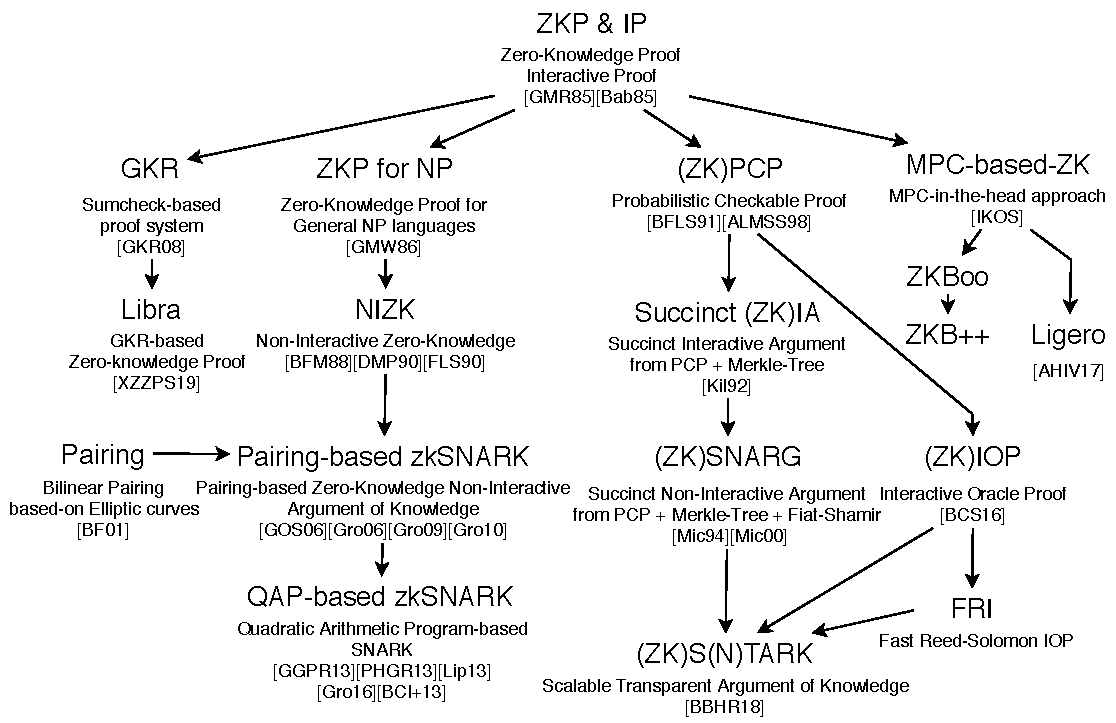
\includegraphics[width=0.5\textwidth]{images/zksnark-history.pdf}
\caption{A Summary of zkSNARK History}
\label{fig:history}
\Description{}
\end{figure}

\paragraph{Theoretical results and challenges.}
We provide definitions for the concepts related to zkSNARKs (Sect.~\ref{sec:proof.system} to \ref{sec:zksnark}), starting from general concepts e.g., proof systems, NP languages, to variations of zkSNARKs, e.g., preprocessing zkSNARK, transparent zkSNARK.
Based on these definitions, we illustrate the theoretical results (Sect.~\ref{sec:security}), including widely believed assumptions and proved theorems.
We intuitively explain why these statements are true, or widely believed to be correct, and refer to the literature for readers interested in the proof details.
We also point out the challenges and open problems in zkSNARKs.

\paragraph{Building tools.}
We describe the toolset used in the existing zkSNARK constructions (Sect.~\ref{sec:build.tool}).
We focus on describing the syntax and properties of the tools, i.e., how to use them and what to expect from them.
We also mention the ideas to realize some tools, for example, the Merkle-Tree as a realization of vector commitment.
We refer to the literature for readers interested in the details of how to construct these tools.

\paragraph{Existing constructions.}
We start describing the existing zkSNARK constructions (Sect.~\ref{sec:construction}) by explaining existing frameworks in the literature (Sect.~\ref{sec:framework}) that try to unify these constructions.
However, none of these frameworks covers the entire state-of-the-art.

We build a new framework by noticing that all zkSNARKs are essentially determined by how they address the following issues:
\begin{itemize}
	\item Which NP-Complete problem to choose;
	\item What is the underlying interactive model;
	\item How to simulate the verifier randomness unpredictably;
	\item How to compress the prover message;
	\item How to save the verifier computation.
\end{itemize}

We then describe the current constructions grouped according to the research branches they reside in:
\begin{itemize}
	\item PCP-based zkSNARKs (Sect.~\ref{sec:pcp.based})
	\item Pairing-based zkSNARKs (Sect.~\ref{sec:pairing.based})
	\item IP-based zkSNARKs (Sect.~\ref{sec:ip.based})
	\item Recursive zkSNARKs (Sect.~\ref{sec:recursive})
\end{itemize}
We position each branch and the inside constructions into our framework by illustrating how they address the issues we mentioned above.
For each construction, we provide a simplified version of the algorithms, and refer to the original literature for details.

\paragraph{Analysis and comparison.}
We address the issue that most zkSNARK users care about: how to select a suitable zkSNARK construction for a particular task?
For this question, we summarize the properties in three groups: efficiency, security, and functionality, as shown in Table~\ref{tab:measure}.

For efficiency properties, e.g., verifier complexity, the property values are expressed as asymptotic functions in some parameters, e.g., the security parameter, the length of the NP witness instance.
For other properties, we enumerate and explain the possible values.
For example, the possible values for ``universality'' include: universal, bounded-size universal, updatable, circuit-specific, parallel-circuit-only.

We list all the property values for each zkSNARK construction.
We also select some application scenarios.
For each scenario, we discuss which properties are most important, and suggest some constructions that are suitable for this scenario.

\begin{table}[tb]
	\caption{Measurement metrics for zkSNARKs}
	\label{tab:measure}
	\centering

	\begin{tabular}{ll}
	\hline

	\hline
	\textbf{Group} & \textbf{Properties} \\
	\hline
	\textbf{Efficiency} & Prover complexity \\
	& Verifier complexity \\
	& Setup complexity \\
	& Proof length \\
	& CRS length \\ \hline
	\textbf{Security} & Zero-knowledgeness \\
	& Trusted setup \\
	& Post-quantum security \\
	& Cryptographic assumption \\ \hline
	\textbf{Functionality} & Expressiveness \\
	& Public verifiability \\
	& Universality \\
	& (Non)Preprocessing \\
	\hline

	\hline
	\end{tabular}
\end{table}


\section{Related Works}

\section{A Biography of zkSNARK}
\label{sec:history}

The zkSNARKs are variations of \emph{zero-knowledge proofs (ZKP)} that originated from the ground-breaking work by Goldwasser, Micali, and Rackoff~\cite{GoldwasserMR85}.
Zero-knowledge proofs are protocols allowing a party, called the prover, to prove a statement to another party, called the verifier, interactively without leaking secret information.
This work also introduced the broader concept of \emph{interactive proofs}, which was simultaneously and independently proposed in the work of Babai~\cite{Babai85} in the name of Arthur-Merlin (AM) proofs.
The major difference between AM proofs and interactive proofs is that AM proofs are public-coin proofs, which means all randomnesses the verifier uses must be revealed later to the prover.

All the precursors of zkSNARKs, including zkSNARKs themselves, can be viewed as special cases of \emph{interactive proofs} with different property combinations.
Particularly, non-interactive proofs are special interactive proofs where the interaction consists of a single message.
For clarity, we prefer to use the term \emph{proof systems} for this broader concept, and refer to interactive proofs only when the interaction contains at least two messages from different parties.

Zero-knowledge proofs demonstrated wide applications~\cite{GoldreichMW86, GoldreichMW87} soon after proposition.
However, the zero-knowledge proof scheme provided by Goldwasser et al.\ is only of theoretical interest and not practical for real-world applications.
Followup works focused on two goals: improving the efficiency to achieve \emph{succinct} interactive proofs, and constructing non-interactive zero-knowledge (NIZK) schemes.
Succinctness means the communication cost and optionally the verifier computation cost are lower than the case when the prover directly reveals the witness to the verifier.

The first breakthrough in improving the efficiency is the proposition of the \emph{Probabilistically Checkable Proof (PCP)} model by Babai et al~\cite{BabaiFLS91}.
The PCP model allows the prover to send to the verifier a proof oracle that the verifier can query probabilistically, instead of a complete proof string that the verifier must read in the whole.
This additional power makes constructing succinct PCP easier than constructing succinct interactive proofs.
The PCP theorem~\cite{AroraLMSS98} later proved by Arora et al.\ indicates the existence of succinct PCPs for any NP languages.

However, the PCP is only an ideal model as the proof oracle is unrealistic to implement.
Regarding this issue, Kilian proposed a method to transform any PCP into a four-message interactive proof~\cite{Kilian92} using cryptographic tools, including collision-resistant hash functions and Merkle-trees.
Kilian's construction is zero-knowledge if the underlying PCP is zero-knowledge.
Meanwhile, the introduction of cryptography restricts the security to hold only against computationally bounded provers, since all-powerful provers can successfully cheat the verifier with false statements by breaking the hash function.
Proof systems with this relaxed security requirement are called \emph{argument systems}~\cite{BrassardCC88}.

For the other goal regarding non-interactivity, Blum et al.~\cite{BlumFM88} showed that NIZK is possible if the prover and the verifier are assumed to share a common random string before the prover generates any proofs.
They also proposed the first NIZK, under the computational assumption that products of two large primes are indifferentiable from products of three large primes.
Furthermore...

\section{Definitions and Theoretical Results}

The zkSNARKs are special proof systems satisfying a specific set of properties.
We first give the definitions of proof systems and several properties that a proof system may have.
Then we define zkSNARKs by referring to these definitions.
Finally, we discuss the theoretical results about different properties of proof systems and demonstrate the minimum assumptions underlying desired combinations of properties.

\subsection{Notations}

We use $\cR$ for an NP relationship, i.e. a set of pairs $\{(x,w):f(x,w)=0\}$ where $x$, $w$ are bit strings of size $n$ and $f$ is a deterministic polynomial-time algorithm.
The NP language $\cL$ induced from $\cR$ is the set $\{x:\exists (x,w)\in\cR\}$.
For $(x,w)\in\cR$, we say $x$ is an instance of $\cL$ and string $w$ is a witness of the fact $x\in\cL$.

We say a system has $\lambda$-bit security if breaking this system costs at least $2^{\lambda}$ units of computation power.
We use $n$ for the bit-lengths of algorithms inputs.
We use $\eta(n)$ for a negligible function in $n$, $\polylog(n)$ for a poly-logarithmic function, and $\poly(n)$ for a polynomial function.
We say an algorithm is p.p.t. if the algorithm is probabilistic and can only execute for a period of length $\poly(n)$.

\subsection{Proof systems}
\label{sec:proof.system}

A proof system is a protocol that allows a party, namely the prover, to prove a statement to another party, namely the verifier.

\paragraph{Statements.} Proof systems usually deal with two types of statements related to an NP language $\cL$:
\begin{enumerate}
	\item given string $x$, the statement claims that $x\in\cL$;
	\item given string $x$, the statement claims knowledge of $w$ such that $(x,w)\in\cR$.
\end{enumerate}

\paragraph{Syntax.}
Given an NP language $\cL$, a proof system $\PiL$ consists of three algorithms $(\Setup,\Prove,\Verify)$.
\begin{enumerate}
	\item $\Setup(\pp)\to(\sigma_P,\sigma_V)$. The $\Setup$ algorithm takes public parameters $\pp$ as inputs and generates reference strings $\sigma_P$ and $\sigma_V$ for the prover and the verifier respectively.
	The reference strings $\sigma_P$ and $\sigma_V$ may intersect with each other, in which case, the intersection is called a \emph{common reference string (CRS)}.
	The $\Setup$ algorithm must be executed before any instance of $\Pi$ can start.
	\item $\langle\Prove(\sigma_P, x, w)\rightleftharpoons\Verify(\sigma_V, x)\rangle\to 0/1$.
	Given a pair $(x,w)\in\cR$, the $\Prove$ algorithm takes a pair $(x,w)$ and the reference string $\sigma_P$ as inputs.
	The $\Verify$ algorithm takes $x$ and the reference string $\sigma_V$ as inputs.
	When being executed, the algorithms may exchange messages between each other.
	Finally, the $\Verify$ algorithm outputs 0 or 1, which is regarded as the output of this protocol.
\end{enumerate}
The execution of a proof system is illustrated in Fig.~\ref{fig:proof.system}.
\begin{figure}[ht!]
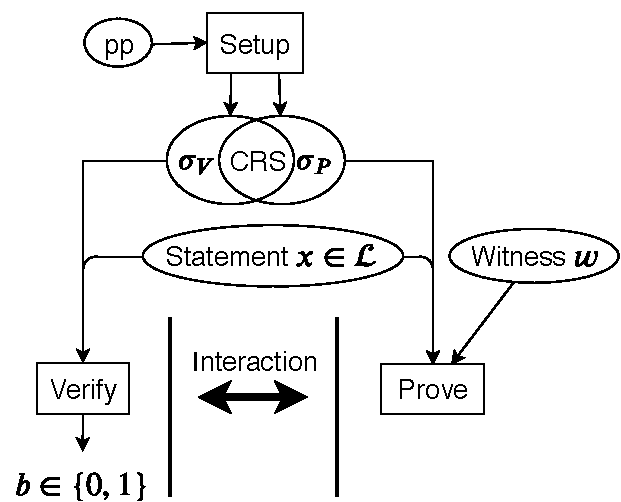
\includegraphics[width=0.3\textwidth]{images/proof-system.pdf}
\caption{Proof System}
\label{fig:proof.system}
\descriptionlabel{An example of a proof system execution.
The rectangles represent algorithms.
The ovals represent inputs to these algorithms.}
\Description{}
\end{figure}


\paragraph{Properties.}
A proof system $\PiL=(\Setup,\Prove,\Verify)$ is expected to satisfy the following properties:

\begin{definition}[Completeness]
\label{def:completeness}
A proof system $\PiL=(\Setup,\Prove,\Verify)$ has \emph{completeness} if for any $(x,w)\in\cR$, correctly executing the protocol always outputs $1$, i.e.
	\begin{eqnarray}
	\Pr\left[b=1\left|
	\begin{matrix}
	\Setup(\pp)\to(\sigma_P,\sigma_V);\\
	\langle\Prove(\sigma_P, x, w)\rightleftharpoons\Verify(\sigma_V, x)\rangle\to b
	\end{matrix}
	\right.\right]=1
	\end{eqnarray}
\end{definition}

\begin{definition}[Soundness]
\label{def:soundness}
	A proof system $\PiL=(\Setup,\Prove,\Verify)$ has \emph{soundness} if for any $x\notin\cL$, for any adversary $\cA$ acting as the prover, the protocol outputs $1$ with probability $\epsilon < 1/2$, where $\epsilon$ is called the soundness error of $\PiL$.
	\begin{eqnarray}
	\label{eqn:soundness}
	\Pr\left[b=1\left|
	\begin{matrix}
	\Setup(\pp)\to(\sigma_P,\sigma_V);\\
	\langle\cA(\sigma_P, x)\rightleftharpoons\Verify(\sigma_V, x)\rangle\to b
	\end{matrix}
	\right.\right]=\epsilon < 1/2\,
	\end{eqnarray}
	If equation (\ref{eqn:soundness}) holds only for p.p.t. adversaries $\cA$, we say $\PiL$ has \emph{computational soundness}.
	In this case, we say $\PiL$ is an \emph{argument system}.
\end{definition}

Note that given $\PiL$ with non-negligible soundness error $\epsilon < 1/2$, we can always construct $\PiL'$ with exponentially small soundness error $\epsilon'$, by repeating the protocol a polynomial number of times.
Therefore, requiring the soundness error to be smaller than $1/2$ is sufficient for a proof system to be useful in practice.

\paragraph{Variations.}
Based on the standard definitions described above, proof systems may take variations in many aspects.
\begin{enumerate}
	\item \emph{Proof-of-knowledge.} Informally, a proof system is said to have proof-of-knowledge, if Definition~\ref{def:soundness} holds not only for $x\notin\cL$, but also for $x\in\cL$ if the adversary does not ``know'' any witness of $x$.
	The notion ``knowledge'' is formally defined by an extractor algorithm.
	\begin{definition}[Proof-of-Knowledge]
	\label{def:proof.of.knowledge}
	A proof system $\PiL=(\Setup,\Prove,\Verify)$ has \emph{proof-of-knowledge} if for any $x\in\{0,1\}^n$, for any adversary $\cA$ acting as the prover, there exists a negligible function $\eta(n)$ and an extractor $\Ext^{\cA}$ which has non-blackbox access to the adversary, such that whenever the adversary successfully cheats the verifier into outputing $1$, $\Ext^{\cA}$ outputs a witness $w$ s.t. $(x,w)\in\cR$ with overwhelming probability, i.e.
	\begin{eqnarray}
	\label{eqn:proof.of.knowledge}
	\Pr\left[
		\begin{matrix}
		b=1\wedge \\
		(x,w)\notin\cR
		\end{matrix}
	\left|
		\begin{matrix}
		\Setup(\pp)\to(\sigma_P,\sigma_V);\\
		\langle\cA(\sigma_P, x)\rightleftharpoons\Verify(\sigma_V, x)\rangle\to b;\\
		\Ext^{\cA}(\sigma_P, x)\to w
		\end{matrix}
	\right.\right]=\eta(n)\,
	\end{eqnarray}
	If equation (\ref{eqn:proof.of.knowledge}) only holds for computationally bounded adversaries, we say the proof system has \emph{argument-of-knowledge}.
	\end{definition}

	\item \emph{Zero-knowledge.} A proof system is said to be zero-knowledge if the verifier cannot extract any ``knowledge'' from the interaction transcripts, i.e. the collection of all the messages sent during the protocol execution.
	The zero-knowledge property is formally defined by a simulator algorithm.
	\begin{definition}[Zero-knowledgeness]
	\label{def:zero.knowledge}
	Let $\tr=[\Prove(\sigma_P, x)\rightleftharpoons\Verify(\sigma_V, x)]$ be the interaction transcript between the prover and the verifier, and call $(\sigma_V,\tr)$ the view of the verifier.
	A proof system $\PiL=(\Setup,\Prove,\Verify)$ is zero-knowledge if for any adversary $\cA$ acting as the verifier, there exists a simulator $\Sim(\cdot)$ such that for any $(x,w)\in\cR$, $\Sim(x)$ is indifferentiable from the view of $\cA$ during the protocol execution, i.e. there exists negligible function $\eta(n)$, s.t. for any differentiator $\cD$:
	\begin{eqnarray}
	\label{eqn:zero.knowledge}
	\left|
	\begin{matrix}
	\Pr\left[
		\begin{matrix}
		\cD(\sigma_V,tr)=1
		\end{matrix}
	\left|
		\begin{matrix}
		\Setup(\pp)\to(\sigma_P,\sigma_V);\\
		[\Prove(\sigma_P, x)\rightleftharpoons\cA(\sigma_V, x)]\to \tr
		\end{matrix}
	\right.\right]\\\\
	-\Pr\left[
		\begin{matrix}
		\cD(\sigma_V,tr)=1
		\end{matrix}
	\left|
		\begin{matrix}
		\Sim(x)\to(\sigma_V,tr)
		\end{matrix}
	\right.\right]
	\end{matrix}
	\right|=\eta(n)
	\end{eqnarray}

	\end{definition}
	The definition of zero-knowledge has some variations.
	\emph{Honest-verifier zero-knowledge} ...
	\emph{Unconditional zero-knowledge} or \emph{perfect zero-knowledge} ...
	\emph{Statistical zero-knowledge} ...
	\emph{Computational zero-knowledge} ...

	\item \emph{Interaction models.} A standard proof system only admits normal interactions, i.e. the prover and the verifier send messages to each other, and each message is read in the whole by the receiver...

	\emph{Non-interactive} ...
	\emph{Probabilistically Checkable Proof (PCP)} ...
	\emph{Interactive PCP (IPCP)} ...
	\emph{Linear PCP (LPCP)} ...
	\emph{Interactive Oracle Proof (IOP)} ...

\end{enumerate}

\emph{Efficiency.} The efficiency of a proof system is measured by the efficiency of each of the algorithms $(\Setup,\Prove,\Verify)$, sizes of the reference strings $(\sigma_P,\sigma_V)$, and the communication cost...

\begin{definition}[Succinctness]
\label{def:succinctness}
A proof system $\PiL$ is succinct if the communication cost of $\PiL$ is at most polylogarithmic to the witness size.
\end{definition}

\begin{definition}[Scalability]
\label{def:scalability}
A proof system $\PiL$ is scalable if...
\end{definition}

\subsection{zkSNARK}
\label{sec:zksnark}

With the above definitions on proof systems and their properties, we can now define zkSNARKs.

\begin{definition}[zkSNARK]
A \emph{zkSNARK} is a proof system that is zero-knowledge (Definition~\ref{def:zero.knowledge}), succinct (Definition~\ref{def:succinctness}), non-interactive, and argument-of-knowledge (Definition~\ref{def:proof.of.knowledge}).
\end{definition}

Depending on how $\Setup$ works, a zkSNARK may be in one or more of the following models.

\paragraph{Preprocessing.} A zkSNARK is called \emph{preprocessing} if ...

\paragraph{Universal setup.} A zkSNARK has \emph{universal setup} if ...

\paragraph{Transparent setup.} A zkSNARK has \emph{transparent setup} if ...

\subsection{Security Assumptions}
\label{sec:security}

After the introduction of zero-knowledge proofs by Goldwasser et al.~\cite{GoldwasserMR85}, Goldreich, Micali, and Wigderson showed that zero-knowledge proofs exist for any NP languages, under the assumption that one-way function exists~\cite{GoldreichMW86}.
The existence of one-way functions is almost the weakest assumption in cryptography.
The only weaker one is P$\neq$NP.
It is also proved that statistical ZK proofs (i.e., both ZK and soundness are statistical) are impossible for NP-complete languages unless P=NP~\cite{AielloH87, Fortnow87, Passs05}.
Therefore, considering general NP languages, at least one side---ZK or soundness---must be computational.
In the interactive case, it is demonstrated that both flavors exist: statistical ZK with computational soundness, or statistical soundness with computational ZK~\cite{BrassardCC88, BrassardC86, GoldreichMW86}.

In the non-interactive case, NIZK constructions only had computational ZK until ...

Succinctness is another property that poses stronger security assumptions on the proof system.
Succinctness is only possible for argument systems, i.e. proof systems with only computational soundness~\cite{BoppanaHZ87, GoldreichH98, GoldreichVW02, Wee05}.
We provide an intuitive proof for the nonexistence of succinct statistically-sound proof systems for NP-complete language $\cL$.
Recall that succinct proof systems have only $O(\log n)$ computation cost where $n$ is the size of NP witness $w$.
If a succinct proof system is also statistically-sound, i.e. it is secure against unbounded prover, the prover should not be able to find valid responses with probability over $1/2$.
Since the prover can search through the entire response space, this means valid responses do not exist at all.
However, that would facilitate a probabilistic $O(n)$ algorithm $\cA$ deciding the language $\cL$ with error $1/2$: for any $x\in\cL$, $\cA$ randomly sample the verifier challenges, loop through the response space in $O(n)$ time, and if $\cA$ does not find any valid response, $\cA$ outputs $0$.
Therefore, $\cL$ is a degenerated language in BPP, i.e. languages having p.p.t. deciding algorithms, which would indicate the collapse of the polynomial hierarchy.
Hence we proved succinct statistically-sound proof systems should not exist for any interesting NP problems.

Furthermore, ...

Table~\ref{tab:security.assumption} summarizes the minimum security assumptions underlying different proof systems.

\begin{table}[tb]
	\caption{Security Assumptions for Different Proof Systems}
	\label{tab:security.assumption}
	\centering

	\begin{tabular}{ccccccc}
	\hline

	\hline
	\textbf{Name} & \textbf{Inter.} & \textbf{ZK} & \textbf{Succ.} & \textbf{Sound} & \textbf{Assum.} & \textbf{Model} \\
	\hline
		NP          & $\times$     & $\times$     & $\times$     & Uncond. & None       & Std. \\
		IP          & $\checkmark$ & $\times$     & $\times$     & Stat.   & None       & Std. \\
		ZKP         & $\checkmark$ & $\checkmark$ & $\times$     & Stat.   & OWF        & Std. \\
		NIZK        & $\times$     & $\checkmark$ & $\times$     & Stat.   & TDP        & CRS \\
		sARG        & $\checkmark$ & $\times$     & $\checkmark$ & Comp.   & CRH        & Std. \\
		sZKA        & $\checkmark$ & $\checkmark$ & $\checkmark$ & Comp.   & CRH        & Std.\\
		sNIZK       & $\times$     & $\checkmark$ & $\checkmark$ & Comp.   & CRH        & CRS / RO \\
		SNARG       & $\times$     & $\times$     & $\checkmark$ & Comp.   & nonf.      & CRS / RO  \\
		SNARK       & $\times$     & $\times$     & $\checkmark$ & AoK     & nonf.      & CRS / RO \\
		zkSNARK     & $\times$     & $\checkmark$ & $\checkmark$ & AoK     & nonf.      & CRS / RO  \\
	\hline

	\hline
	\end{tabular}
\end{table}


\section{Building Tools}
\label{sec:build.tool}

Here we illustrate some tools in cryptography and computation complextiy theory that zkSNARKs are built on.

\subsection{Commitment scheme}
\label{sec:commitment}

A cryptographic commitment scheme enables ...
A commitment scheme is a tuple $\Gamma=(\Setup, \Comm, \Open)$ of p.p.t. algorithms.
\begin{enumerate}
	\item $\Setup(1^{\lambda})\to\pp$ generates public parameters given the security bit number
	\item $\Comm(\pp,m)\to(\cm,r)$ takes a message $m$ and generates a commitment $\cm$, together with an opening hint $r$
	\item $\Open(\pp,\cm,m,r)\to b\in\{0,1\}$ takes a message $m$, a commitment $\cm$ and an opening hint $r$, and verifies if $\cm$ is a valid commitment of $m$.
	If $b=1$, we say $(m,r)$ is a correct opening of $\cm$.
\end{enumerate}
A commitment scheme is expected to be \emph{binding}.

\begin{definition}[Binding]
A commitment scheme $\Gamma=(\Setup,\Comm,\Open)$ is binding if ...
\end{definition}

A commitment scheme can optionally be \emph{hiding}.

\begin{definition}[Hiding]
A commitment scheme $\Gamma=(\Setup,\Comm,\Open)$ is hiding if ...
\end{definition}

\paragraph{Polynomial commitment.} Polynomial commitment schemes are variants of commitment schemes that have message space $R[X]$, i.e. polynomials over ring $R$, and allow opening a single evaluation of the committed polynomial~\cite{KateZG10}.
A polynomial commitment scheme is a tuple $\Gamma=(\Setup,\Comm,\Open,\Eval)$ where $(\Setup,\Comm,\Open)$ is a commitment scheme and $\Eval(\pp,\cm,x,y,d)\to b\in\{0,1\}$ is a protocol ...
Except for the binding and hiding properties, a polynomial commitment scheme $\Gamma$ is also expected to be \emph{correct} and \emph{evaluation binding}.

\begin{definition}[Correct]
A polynomial commitment sheme $\Gamma=(\Setup,\Comm,\Open,\Eval)$ is correct if ...
\end{definition}

\begin{definition}[Evaluation binding]
A polynomial commitment sheme $\Gamma=(\Setup,\Comm,\Open,\Eval)$ is evaluation binding if ...
\end{definition}

Sometimes we need a stronger property than the evaluation binding called \emph{knowledge soundness} that requires the prover to ``know'' the committed polynomial~\cite{BunzFS20}.

\begin{definition}[Knowledge soundness]
A polynomial commitment sheme $\Gamma=(\Setup,\Comm,\Open,\Eval)$ has knowledge soundness if ...
\end{definition}

\paragraph{Accumulator.}
Accumulators are another kind of variations of commitment schemes.
Instead of committing a single element, an accumulator allows committing to a list of elements, and ...

Merkle-tree is an example of an accumulator ...

\subsection{Fiat-Shamir transformation and random oracle}
\label{sec:fiat.shamir}

Fiat-Shamir transformation is the standard way to transform a public-coin interactive protocol to a non-interactive scheme.
The Fiat-Shamir transformation works by simulating the verifier challenges by the hash value of prover messages.
However, the security of the resulting non-interactive scheme is established only in the random oracle model.
Current security proving techniques require modeling the hash function by a random oracle, which is an ideal functionality that does not exist in reality.

A random oracle is ...

\subsection{Bilinear pairing}
\label{sec:pairing}

Given groups $\bbG_1$, $\bbG_2$ and $\bbG_T$, with $|\bbG_1|=|\bbG_2|=|\bbG_T|=q$, a bilinear pairing~\cite{BonehF01} is a mapping $e:\bbG_1\times\bbG_2\to\bbG_T$ that satisfies...

\section{Existing zkSNARK Constructions}
\label{sec:construction}

Having introduced the theoretical definitions, we are ready to investigate the details of current constructions.

\subsection{Construction Framework}
\label{sec:framework}

Before explaining the details, it would be convenient to put the various constructions into a common framework.
We will briefly review the existing frameworks and demonstrate our unified framework.

B\"{u}nz et al.~\cite{BunzFS20} proposed a framework by noting that many SNARKs can be obtained by compiling a polynomial IOP with a polynomial commitment scheme and the Fiat-Shamir protocol.
A polynomial IOP is an IOP where the proof oracles are restricted to a polynomial, i.e. an oracle that responses with $f(x)$ at query $x$ for some polynomial $f$ of bounded degree.
The polynomial commitment scheme is responsible for ensuring the prover to behave like a polynomial oracle.

The ZKProof Community in a reference document~\cite{ZKProof20} presents a more general framework saying that all the ZKPs are obtained by applying a cryptographic transformation to an information-theoretic proof system.

Ben-Sasson recently showed another perspective to view all cryptographic proofs, not just zkSNARKs, as a combination of an \emph{arithmetization} method and a polynomial \emph{low degree checking (LDC)} scheme~\cite{Ben-Sasson2020}.
The arithmetization step transforms a computation satisfaction problem into an algebraic problem that is more friendly with proof systems.
The algebraic problem is usually described as a polynomial equation.
The low degree checking step verifies that the polynomials provided by the prover are within appropriate degree limits.

These different frameworks focus on different parts of the same zkSNARK construction pipeline, illustrated in Fig.~\ref{fig:pipeline}.
B\"{u}nz et al.~\cite{BunzFS20} focuses on abstracting all the proof systems with polynomial IOP and the first compilation into argument systems.
Ben-Sasson~\cite{Ben-Sasson2020} focuses on arithmetization and views the other three steps in the whole as an LDC scheme.

\begin{figure}[ht!]
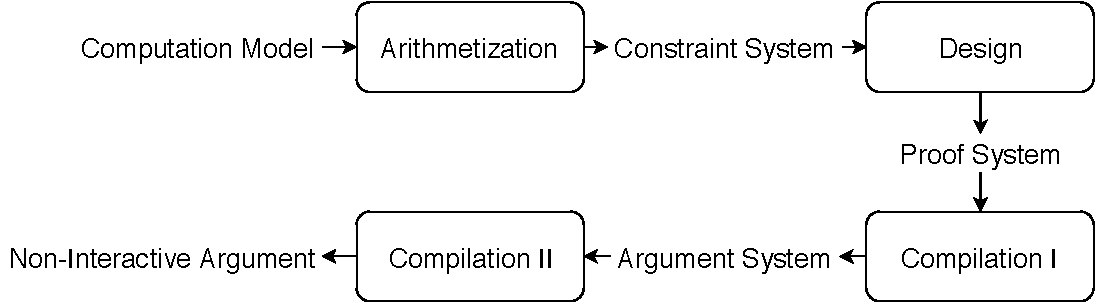
\includegraphics[width=0.5\textwidth]{images/pipeline.pdf}
\caption{zkSNARK Construction Pipeline}
\label{fig:pipeline}
\Description{}
\end{figure}

We propose a new framework based on this pipeline, ...

We will introduce the current zkSNARK constructions grouped by the research lines.
In each group, we will extract the common techniques they share and dive into the details of their differentiations ...

\subsection{PCP-based zkSNARKs}
\label{sec:pcp.based}

The PCP-based approach is the result of the series of works of Blum et al.~\cite{BabaiFLS91}, Kilian~\cite{Kilian92}, and Micali~\cite{Micali00}.
The idea is to design a ZK-PCP for the given language, then compile it into a succinct interactive argument using a commitment scheme~\cite{Kilian92}, and finally apply the Fiat-Shamir transformation to obtain a zkSNARK~\cite{Micali00}.
For those zkSNARKs based on generalizations of ZK-PCP, e.g. ZK-IPCP, ZK-IOP, we also categorize them into this group.

Most of the researches in this category focus on the design of ZK-PCP.
Therefore, they mainly differ in the arithmetization and proof system design.
Another two lines of work fall into this category: the Multi-Party Computation (MPC)-based, and the Polynomial IOP (PIOP)-based zkSNARKs.

\paragraph{STARK.}

\paragraph{Aurora.}

\paragraph{Fractal.}

\subsubsection{MPC-based zkSNARKs}
\label{sec:mpc.based}

The MPC-based approach presents a way to transform a secure multi-party computation for any NP language into a ZK-IPCP.
This line of work originated from Ishai, Kushilevitz, Ostrovsky, and Sahai (IKOS)~\cite{IshaiKOS07}, ...

A multi-party computation scheme is ...

\paragraph{ZKBoo}

\paragraph{ZKB++}

\paragraph{Ligero}

\subsubsection{PIOP-based zkSNARKs}
\label{sec:piop.based}

\paragraph{Sonic}

\paragraph{PLONK}

\paragraph{Supersonic}


\subsection{Pairing-based zkSNARKs}
\label{sec:pairing.based}

The pairing-based zkSNARKs have one of the most efficient verifier and the smallest proof size.
As a sacrifice, they rely on an expensive per-circuit trusted setup.
This line of research originated from the series of works by Groth, Ostrovsky, and Sahai~\cite{GrothOS06Non, GrothOS06Perfect, Groth10}, after the introduction of bilinear-pairing by Boneh et al.~\cite{BonehF01}.

\paragraph{GGRP13.}

\paragraph{Pinocchio.}

\paragraph{BCGTV13.}

\paragraph{Groth16.}

\subsection{IP-based zkSNARKs}
\label{sec:ip.based}

The interactive proof (IP)-based line of research started from the Muggles paper~\cite{GoldwasserKR08} by Goldwasser et al. that brings the GKR protocol.
However, these studies did not produce a zkSNARK until T. Xie et al. proposed Libra~\cite{XieZZPS19} which introduces the zero-knowledge property to GKR.

To learn about the Libra zkSNARK, it is inevitable to first introduce the famous sum-check protocol, which is the foundation of GKR protocol.

\paragraph{The Sumcheck protocol.}

\paragraph{The GKR protocol.}

\paragraph{Libra.}

\subsection{Recursive zkSNARKs}
\label{sec:recursive}

The recursive technique is based on the insight that we can further verify the zkSNARK verification computation recursively by another zkSNARK.
Recursive zkSNARKs work with two primitives: proof-carrying data (PCD) and bootstrapping...

\section{Analysis and Comparison}
\label{sec:analysis}

Evaluating and comparing the zkSNARK constructions is challenging because of the high dimensionality of metrics.
To mitigate this problem, we categorize these metrics into three groups: efficiency, security, and functionality.
Instead of presenting all the dimensions simultaneously as efficiency analysis usually does, we design several real-world application scenarios.
Each scenario specifies two sets of criteria: the hard criteria filter for zkSNARKs that satisfy given conditions, and the soft criteria define an order over these filtered zkSNARKs.

\subsection{Computation Delegation}

A common application of zkSNARKs is computation delegation.
In this scenario, the verifier is usually a device with weak computation power, e.g. a smartphone, while the prover has much more computational resources, e.g. a cloud server.
The verifier may delegate computation tasks to the prover, but the prover is not completely trustable.
In this case...

\subsection{Organization with Authorized Leader}

\subsection{Value-transfer-only Permissionless Blockchain}

In a permissionless blockchain, if most activities are transfers of currency ownerships, e.g. in Bitcoin or Zerocash, the verifier efficiency, the proof size, and the public verifiability are crucial.
Meanwhile, other properties e.g. high prover efficiency, post-quantum security, transparency are nice but not fate-determining.
Expressiveness and universality are less interesting as the blockchain functionality is simple and stable.
In this case...

\subsection{Permissionless Blockchain with Smart Contract}

In permissionless blockchains supporting Turing complete smart contracts, e.g. Ethereum, Nervos, the verifier efficiency, the proof size, and the public verifiability are as important as in value-transfer-only blockchains.
Meanwhile, expressiveness and universality are as significant as efficiency...


\section{Conclusion}

We recalled the history of zkSNARKs and summarized the knowledge of zkSNARKs in three levels: the theoretical level, the technical level, and the application level.
At the theoretical level, by recalling the history, we introduced the proof systems and presented a definition for zkSNARKs in this broader context.
To better understand the zkSNARK constructions, we demonstrated the theoretical results about proof systems and zkSNARKs, e.g. the security assumptions required for different combinations of efficiency and functionality.
At the technical level, we introduced existing zkSNARK construction frameworks and presented a unified framework.
We provided the details of different zkSNARK research lines in the perspective of this framework.
Finally, at the application level, we analyzed and compared the zkSNARKs in terms of efficiency, security, and functionality, in different application scenarios.

\bibliographystyle{unsrt}
\bibliography{reference}

\end{document}